\documentclass[conference]{IEEEtran}
\IEEEoverridecommandlockouts

\usepackage{booktabs} % For formal tables
\usepackage{graphicx}
%\usepackage[position=b]{subcaption}
\usepackage[hyphens,spaces,obeyspaces]{url}
%\usepackage{multicol,tabularx,capt-of}
\usepackage{multicol}
\usepackage{multirow}

%\usepackage{hyperref}

% Make it ok to have lines that don't span the whole text width in the bibliography.
%\usepackage{etoolbox}
%\apptocmd{\thebibliography}{\raggedright}{}{}

%\usepackage{breakurl}
% correct bad hyphenation here
%\hyphenation{op-tical net-works semi-conduc-tor}


\begin{document}


% Titles are generally capitalized except for words such as a, an, and, as,
% at, but, by, for, in, nor, of, on, or, the, to and up, which are usually
% not capitalized unless they are the first or last word of the title.
% Linebreaks \\ can be used within to get better formatting as desired.
% Do not put math or special symbols in the title.
\title{Maverick: A Stand-alone CAD Flow for Partially Reconfigurable FPGA Modules}
% Does IEEE have a special format they want me to use for funding? (ACM had strict requirements))


% author names and affiliations
% use a multiple column layout for up to two different
% affiliations


\author{\IEEEauthorblockN{Dallon Glick, Jesse Grigg, Brent Nelson, Michael Wirthlin}
	\IEEEauthorblockA{
		{NSF Center for Space, High-Performance, and Resilient Computing (SHREC)} \\
		{Department of Electrical and Computer Engineering} \\
		{Brigham Young University}\\
		Provo, UT, 84602, USA \\
		\{dallon.glick, grigg.jesse, brent\_nelson, wirthlin\}@byu.edu}
	\thanks{This work was supported in part by the I/UCRC Program of the National Science Foundation within the NSF center for Space, High-performance, and Resilient Computing (SHREC) under Grant No.~1738550.}
}

% \author{\IEEEauthorblockN{Anonymous Author(s)}
% }

% make the title area
\maketitle

\begin{abstract}
This paper presents Maverick, a proof-of-concept computer-aided design (CAD) flow for generating reconfigurable modules (RMs) which target partial reconfiguration (PR) regions in field-programmable gate array (FPGA) designs.
After an initial static design and PR region are created with Xilinx's Vivado PR flow, the Maverick flow can then compile and configure RMs onto that PR region---without the use of vendor tools. 
Maverick builds upon existing open source tools (Yosys, RapidSmith2, and Project X-Ray) to form an end-to-end compilation flow.
This paper describes the Maverick flow and shows the results of it running on a PYNQ-Z1's ARM processor to compile a set of HDL designs to partial bitstreams.
The resulting bitstreams were configured onto the PYNQ-Z1's FPGA fabric, demonstrating the feasibility of a single-chip embedded system which can both compile HDL designs to bitstreams and then configure them onto its own programmable fabric.
\end{abstract}


\begin{IEEEkeywords}
	Field-programmable gate arrays; Partial reconfiguration; Electronic design automation and methodology; RapidSmith
\end{IEEEkeywords}

% For peer review papers, you can put extra information on the cover
% page as needed:
% \ifCLASSOPTIONpeerreview
% \begin{center} \bfseries EDICS Category: 3-BBND \end{center}
% \fi
%
% For peerreview papers, this IEEEtran command inserts a page break and
% creates the second title. It will be ignored for other modes.
\IEEEpeerreviewmaketitle

\section{Introduction}
\label{sec:introduction}

Partial Reconfiguration (PR) is a technique which allows portions of a field-programmable gate array (FPGA) to be dynamically reconfigured after the complete device has been initially configured.
This allows the circuit's functionality to be customized on the fly, such as in response to changing operating conditions or user directives.
In the most common form, a PR design includes a static region and one or more PR regions into which pre-compiled circuits can be configured at run-time.
The static region contains common and unchanging functionality such as external I/O interfaces, clocking, and other base system functionality.
The PR regions reserve logic for functions which can change dynamically, such as accelerator cores.
As FPGA sizes continue to grow we believe the use of PR will become increasingly important.

Xilinx provides a PR design flow for their FPGA devices \cite{Xilinx:2018d}.
In a basic form of this flow, a base static design is created by the user and a specific module is identified to be partially reconfigurable; this module is known as a reconfigurable module (RM). 
For this RM, a physical PR region (known as a reconfigurable partition in Vivado's PR flow) is identified, into which the RM's circuitry will be placed and routed.
The subsequent tool flow steps then implement the entire design while limiting the RM's circuitry to its defined region.
The result is a full-chip bitstream which can be configured onto the device. 
Later, other RMs can be compiled into the same PR region, resulting in partial bitstreams which can be dynamically reconfigured onto the PR region.

To compile these RMs requires the availability of the original PR project files as well as the full Vivado design suite, no matter how small the RM.
A full Xilinx Vivado 2018.2 installation requires over 50 GB of disk space to support the design of Xilinx FPGAs from several families.
A minimum of 48 GB of RAM is also required to compile designs to bitstreams for the largest devices \cite{Xilinx:2018}.
Additionally, Vivado can only be run on x86 or x86-64 machines \cite{Xilinx:2018b}.
These requirements limit the sizes and types of machines that PR designs can be developed on.

This work introduces a different model for creating PR designs in which the original design is created using Vivado’s PR flow, and subsequent RMs can then be created on-the-fly using lightweight tools, independent of Vivado.
By separating out the initial static design creation from later RM creation, a smaller portion of the FPGA fabric is targeted by the CAD tools, allowing them to run on systems with lower memory, storage, and compute requirements.
This paper describes Maverick, a Vivado-independent RM tool flow, which can be run on a variety of systems, including embedded systems.

The independent and lightweight nature of Maverick opens up a number of new usage models, not readily supported by the current vendor tools.
For example, this enables the creation of fully autonomous systems which are untethered from other compute resources.
In this model, adaptation algorithms running on an autonomous platform could create new HDL design code for an RM (or modify existing RM HDL code) which would then be compiled by the Maverick flow and configured onto the platform's FPGA fabric.
Such autonomous systems could use this model to provide domain specific functionality or to improve fault tolerance.
Another potential usage model is a customized system tailored for education, which could mix instructional materials, sample designs, HDL code, and CAD tools into a lightweight stand-alone hardware platform.
This would enable the creation of a set of specialized visualization and analysis tools for learning on top of that system.

This paper demonstrates the Maverick flow executing on the embedded PYNQ-Z1 board, which contains a Zynq 7020 system on chip (SoC).
The Maverick CAD tools run on an ARM processor embedded within the processing system (PS) of the Zynq device.
This flow generates partial bitstreams which are configured onto a PR region within the programmable logic (PL) fabric of the same Zynq device.

Additionally, this paper reports on the results of several simple benchmark designs compiled on the PYNQ-Z1.
The execution time and memory requirements of the Maverick flow are measured for each design run.
The quality of results of the generated designs within Maverick is also compared against results from the same set of circuits generated by the commercial Vivado tools.
Although the Maverick design flow does not produce circuits with the same level of quality as the commercial tool flow, this paper demonstrates that it is possible to generate usable, operating circuit bitstreams within FPGA PR regions {\em without} the need of any commercial tools.

\section{Related Work}
\label{sec:background}

The Maverick flow is a 3rd party CAD tool flow which targets commercial FPGA devices.
A number of other research projects have also produced tools in this same category, each of which addresses a different subset of the overall FPGA implementation flow.  
The tools most similar to the Maverick flow are described in this section.

Several tools have been introduced which allow for the manipulation of Xilinx designs in various ways.
Torc \cite{Steiner:2011}, RapidSmith \cite{Lavin:2011}, RapidSmith2 \cite{Haroldsen:2015}, and RapidWright \cite{Lavin:2018} all fit into this category---their principal use has been to enable users to perform CAD tasks for Xilinx FPGAs that are not readily possible using vendor tools \cite{Petelin:2016} \cite{Cannon:2018}.
Additionally, the VTR-to-Bitstream \cite{Hung:2015} project demonstrated  a 3rd party flow which implemented several steps of the flow for Xilinx devices.
All of these tools must return their designs to the Xilinx flow for the bitstream generation step.

In contrast, a number of other projects have been created that can generate bitstreams for commercial FPGAs.
The work in \cite{Steiner:2008} describes a proof-of-concept autonomous computing system running on the PowerPC of an embedded Virtex-II Pro device.
This system could place, route, and generate partial bitstreams for technology mapped (tech-mapped) designs. 
For bitstream generation, it used an unreleased version of Xilinx's JBits.

Another toolchain, the IceStorm flow \cite{IceStorm}, is a full FPGA CAD flow for the commercially available iCE40 family of FPGAs from Lattice Semiconductor.
It uses Yosys \cite{Wolf:2013} for synthesis, Arachne-pnr \cite{Arachne-pnr} for placement and routing, and the Project IceStorm tools for bitstream generation.
This flow has enabled Trenz Electronic's icoBoard \cite{icoBoard}, a Raspberry Pi accessory containing an iCE40 FPGA.
Using the icoBoard and a Raspberry Pi board, the IceStorm flow can compile designs to bitstreams on the Raspberry Pi's ARM CPU.
These bitstreams can then be programmed onto the iCE40 FPGA.

We believe that the Maverick work is interesting and novel because it combines the following characteristics.
First, it is a new PR flow which provides a new model for system development by enabling the independent creation of multiple RM designs once a static design has been created.
Furthermore, it is a lightweight CAD flow and can thus run on a single-chip embedded system in minimal memory (our demonstrations show it running in under 250 MB of RAM).
Also, being based on the RapidSmith/RapidSmith2 tool framework, it already supports Xilinx 7-Series devices and is readily extensible to future Xilinx devices such as UltraScale and UltraScale+.
\section{Static Design Phase}
\label{sec:static_system}
The system described in this paper operates in two phases.
The first phase relies on Vivado to create an initial static design and the second phase, the Maverick flow, allows the creation of subsequent RMs, independent of Vivado.
This section describes that first phase, the static design phase.

As shown in \figurename~\ref{fig:static_system}, this phase is made up of three steps to create the full static design.
The full static design consists of a Vivado-generated static design, containing a static region and a PR region, and some associated metadata.
This metadata describes the PR region and its interface with the static region.

\begin{figure}
	\centering
	\includegraphics[height=.68\columnwidth]{figures/static_system.pdf}
	\caption{Static Design Phase}
	\label{fig:static_system}
\end{figure}

\subsection{Static Design Creation: Vivado}
In the first step of the static design phase, a base static design is created and compiled using Vivado's PR flow.
First, the static design HDL, which contains static logic and a black box RM, is synthesized with Vivado's PR flow. 
An initial RM HDL design is then separately synthesized with Vivado's PR flow.

Next, a floorplan is created to define the PR region into which RMs will be physically implemented.
This PR region must be chosen to adhere to certain horizontal and vertical alignment requirements imposed by the device architecture \cite{Xilinx:2018d}.
The initial synthesized RM design is then assigned to this PR region, creating an initial full-device design.

\begin{figure}
	\centering
	\includegraphics[width=.65\columnwidth]{figures/partPins.pdf}
	\caption{A Static Design with Partition Pins and Reserved Resources}
	\label{fig:partPins}
\end{figure}

Vivado's PR flow is then used to place and route this full-device design.
All static logic is constrained to be within the static region of the FPGA, while RM logic is constrained to be within the PR region.
However, some routing resources within the PR region may be used to route static circuitry; these resources are reserved by the static design and cannot be used by RMs.
\figurename~\ref{fig:partPins} shows a static design and represents these reserved routing resources as dashed lines.

Placement and routing also results in the creation of partition pins, which are the logical and physical points at which the static logic and RMs interface.
These partition pins act as top-level ports for the RM designs implemented within the PR region, giving the RM designs access to I/O and other global resources located in the static region.
Partition pins are physically implemented as wire segments within PR regions \cite{Xilinx:2018d}.
Vivado's PR flow creates routes that connect the static logic and the partition pins, as seen in \figurename~\ref{fig:partPins}.
These partition pins and routes are also reserved by the static design and must be consistent across all RMs.

After Vivado's PR flow finishes creating the static design, a bitstream corresponding to the static (base) part of the design is generated; this can be used to pre-configure the FPGA prior to any partial bitstreams being configured onto it.
Next, an initial partial bitstream corresponding to the empty PR region, containing no RM circuitry, is created.
Custom Tcl scripts are then executed within Vivado to generate a list of routing resources that are reserved by the static design and which lie within the PR region.
The Maverick flow needs this list to prevent these resources from being used during the RM implementation stages.
These two pieces of data (bitstreams and reserved resources) are shown in the upper right portion of \figurename~\ref{fig:static_system}.

\subsection{Partial Device Model: RapidSmith2}
RapidSmith2 \cite{Haroldsen:2015} is an open-source FPGA CAD tool framework which provides a design representation and a circuit manipulation API upon which CAD tools can be written. 
The next step in the static design phase is the creation of a {\em partial device model}, which is used by the RapidSmith2-based tools of the Maverick flow.
RapidSmith2 normally creates full device models for its own use by parsing XDLRC files, which describe Xilinx device data in great detail.
For modern Xilinx devices, these XDLRC files are generated using Tincr \cite{White:2014} and the Vivado Design Interface (VDI) \cite{Townsend:2017b}, which together contain a library of Tcl and Java routines to enable the export and import of device and design data.

To create partial device models, a new RapidSmith2-based partial device generator is used.
This partial device model describes only the resources within a specified PR region of a device that are available to the Maverick flow for implementing RM designs.
This includes all the logic slices, clocking resources, interconnect, and other configurable resources within the PR region.
Additionally, this model describes all interconnect resources that can be used to enter or leave the PR region.
Because this partial device model describes only a particular subset of the full FPGA (i.e., the PR region), the memory required to represent the design is greatly reduced.

\subsection{Bitstream Database Generation: Project X-Ray}
The last set of static design metadata that needs to be generated is a Project X-Ray \cite{PrjXray} bitstream database.
Project X-Ray is an open-source project that aims to document the Xilinx 7-Series bitstream format.
Project X-Ray does this by using Vivado's Tcl API to generate bitstreams for several small designs with specific properties.
Several tools are then used to analyze these bitstreams and to map specific device features to specific bits in the bitstream, resulting in a bitstream database.

At the time of the writing of this paper, Project X-Ray generates a bitstream database for a subset of 7-Series device features within a specific region of interest in an Artix7 FPGA.
As a part of our work, we modified several of the Project X-Ray Tcl scripts to support Zynq FPGAs.
This bitstream database in conjunction with the initial partial bitstream (created with Vivado's PR flow) provides the necessary information for the Maverick flow to generate new partial bitstreams for placed and routed designs within the PR region.
At this point, the static design phase is complete and Vivado is no longer needed.

\section{Maverick Flow Phase}
\label{sec:flow}

\begin{figure}[tb]
	\centering
	\includegraphics[height=.8\columnwidth]{figures/maverick_flow.pdf}
	\caption{Maverick Flow Phase}
	\label{fig:maverick_flow}
\end{figure}

The second phase is the stand-alone Maverick flow, which compiles RM designs to the PR region, independently of any vendor tools.
The Maverick flow is shown in \figurename~\ref{fig:maverick_flow} and consists of six major steps: synthesis, packing, placement, routing, FASM (FPGA Assembly) file generation, and bitstream generation.
This section describes each of these steps in turn.

\subsection{Synthesis and Tech-Mapping: Yosys}

\begin{figure}[tb]
	\centering
	\includegraphics[width=0.58\columnwidth]{figures/synthesis}
	\caption{The Synthesis and Tech-Mapping Step in Maverick}
	\label{fig:synthesis}
\end{figure}

The first step of the Maverick flow is synthesis and tech-mapping. 
Maverick performs this using Yosys \cite{Wolf:2013}, a powerful open source framework for register-transfer level (RTL) synthesis that is capable of tech-mapping to Xilinx 7-Series devices. 
\figurename~\ref{fig:synthesis} shows how Yosys is used in the Maverick flow. 

Maverick executes Yosys using a synthesis script that combines several standard Yosys subsystems to optimize and tech-map the RM Verilog design to the Xilinx 7-Series architecture. 
At the time of this work, both Yosys and Project X-Ray support only a subset of 7-Series device features.
Because of this, the synthesis script limits Yosys to mapping designs to slice structures (containing lookup tables [LUTs] and flip-flops) only.
%As support for additional device features is added to these two tools, the entire Maverick flow will be able to support a larger subset of the device.  

Yosys produces a tech-mapped design in the form of a flattened EDIF netlist.
This netlist is made up of logical Xilinx 7-Series cells (e.g., LUTs and flip-flops) that are all interconnected by logical nets.   
The Maverick flow packages the EDIF netlist and the reserved resource list (from the static design) into a RapidSmith Checkpoint (RSCP), which is suitable for processing by RapidSmith2.

\subsection{RapidSmith2 Design Import}
\begin{figure}
	\centering
	\includegraphics[width=0.58\columnwidth]{figures/rs2_steps.pdf}
	\caption{The RapidSmith2-based Steps in Maverick}
	\label{fig:rs2_steps}
\end{figure}

As shown in \figurename~\ref{fig:rs2_steps}, a set of RapidSmith2-based programs are next used to physically implement the tech-mapped design.
The next step in the Maverick flow is thus to import the tech-mapped design from Yosys into RapidSmith2.

To do so, the partial device model (from the static design) is first imported, providing RapidSmith2 with necessary details about the resources available in the PR region. 
The RSCP generated from the previous synthesis and tech-mapping step is also imported.
The EDIF netlist contained in the RSCP is translated for use within RapidSmith2 and the reserved resource list is then parsed to create internal data structures that mark the resources reserved by the static design.

\subsection{Packing: RSVPack}
The Maverick flow next packs the design, grouping related cells from the netlist into relatively placed clusters.
The created clusters correspond to sites in the Xilinx architecture, most of which are slices.
These sites are composed of internal site wires and Basic Elements of Logic (BELs).
These BELs include logic BELs, such as LUTs and flip-flops, and also routing BELs, which are programmable routing muxes.

The Maverick flow packs designs using the RSVPack algorithm \cite{Haroldsen:2016}.
RSVPack specifically targets Xilinx architectures, allowing it to produce results that take advantage of unique architectural features.
The version of RSVPack used in this work has been modified to work within PR regions---specifically to recognize partition pins.

The RSVPack algorithm repeatedly packs the site clusters with cells. 
To ensure that the clusters are valid for the target architecture, a series of tests is run each time a cell is added to a cluster.
Each time a cell is added to a cluster, a series of tests is run to verify that the cluster is valid for the architecture.
After all the cells in the design have been packed, RSVPack performs the intra-site routing of the nets; i.e., it routes all the portions of the nets that are inside the site clusters.
It does this by configuring the site clusters' internal routing BELs.

\subsection{Placement: RSVPlace}
Once packing completes, the Maverick flow places the design using a modified version of RSVPlace \cite{Haroldsen:2016}, also built on top of RapidSmith2. 
%RSVPlace is a non-timing driven placer. 
It first performs a quick random placement of the clusters created in the packing step.
This is followed by the execution of a simulated annealing placer using a wire-length based cost function.
The cost function and annealing schedule used by this placer are both based on VPR's placer \cite{Betz:1997}.
Furthermore, the placer uses the partial device model (created in the static design phase), preventing the placer from using any resources outside the PR region.

As mentioned previously and shown in \figurename~\ref{fig:partPins}, some resources within the PR region may be used by the static region and are marked as reserved.
RSVPlace was modified to not utilize any of these resources.
This is necessary for a PR-aware placer because in some initial static designs produced by Vivado the static logic may use a site within a PR region as a ``route-through''.
When a site is used as a route-through, the entire site is used to route a net from one of the site's input pins to one of its output pins.
Sites used by the static design as route-throughs are thus unavailable for use by the placer.

Once RSVPlace completes, all logical cells of the design have been assigned to specific locations in the PR region.
These assignments are saved internally within RapidSmith2, giving a global router the information it needs to complete the routing of the design.

\subsection{Routing: RSVRoute}
The Maverick flow then uses a new router called RSVRoute, also built upon the RapidSmith2 framework, to route the nets of the design. 
RSVRoute is primarily based on Pathfinder \cite{Ebeling:1995} and is the first full router created using RapidSmith2.
To construct routes, it turns on programmable interconnect points (PIPs) contained within the FPGA interconnect.

RSVRoute iteratively routes the unrouted and congested nets in the design until all nets are routed and uncongested.
Like VPR \cite{Betz:1997}, the cost for a net to use a congested routing resource is the product of the base cost, present congestion penalty, and historical congestion penalty of that routing resource.
Also like VPR, the present congestion penalty of a routing resource is updated every time a net is routed and the historical congestion penalty is updated between routing
iterations.
During every routing iteration, RSVRoute uses the A* shortest path algorithm \cite{Hart:1968} to quickly identify a shortest path, based on wire-length, for each congested net.

RSVRoute has two unique characteristics to support PR.
First, it must create routes while avoiding PIPs that are reserved by the static design. 
Second, in an RM design, nets connect to not only logic block pins but also to partition pins, which are physically implemented as wire segments within the PR region.
RSVRoute interconnects logic block pins with these partition pins; this feature is essential for completing the routing of RM designs contained within PR regions.

\subsection{FASM Generation: RapidSmith2}
\label{sec:fasm}

The next step in the Maverick flow is to generate an FPGA Assembly (FASM) file \cite{PrjXray}.
This is a human-readable text file that contains a list of low-level instructions to configure the FPGA's resources.
Specifically, FASM files contain instructions to perform functions such as enabling PIPs in interconnect tiles, configuring LUTs, and configuring other BEL and site-level properties.
The FASM format contains enough information so that in conjunction with the bitstream database and initial partial bitstream, a new valid partial bitstream can be generated for an RM design.

As shown in \figurename~\ref{fig:rs2_steps}, data structures created by each of the preceding RapidSmith2-based programs are used to generate the FASM file.
Many of the FASM instructions are straightforward to generate due to the detailed partial device model imported into RapidSmith2.
For instance, to determine the interconnect PIPs to turn on, the FASM generator iterates through route tree data structures (created by RSVRoute).
Each time an enabled PIP is encountered, the FASM generator writes a corresponding instruction to the output FASM file.
An example of such an instruction is shown below: 
\begin{center}
	\texttt{INT\_L\_X38Y16.SE2BEG1 LOGIC\_OUTS\_L1}
\end{center}
\noindent In this example, the starting point for the connection to be turned on is the wire ``LOGIC\_OUTS\_L1'', located in the interconnect tile ``INT\_L\_X38Y16'', and the PIP to be turned on is the one which connects that wire to the wire ``SEG2BEG1''. 
It is similarly straightforward to configure routing BELs.

Writing the instructions to configure sites and their logic BELs is more challenging, mainly because EDIF netlists represent only the logical properties associated with the cells in the netlist and not the physical site-wide and BEL properties.
This necessitates the translation of logical properties associated with cells to physical properties associated with sites and BELs.
One example of a property that requires such translation is whether all the flip-flops in a slice use a synchronous or an asynchronous reset.
Another example has to do with LUT programming. 
Routing may reorder a LUT's input pin connections to help with routing congestion; this requires the LUT equation be reformulated.
Additional handling is also necessary for fracturable 6-input LUTs and LUT RAM initialization.
All of this handling must be done in order to produce correct FASM instructions.

An important final step for the FASM generator is to process the resources that were reserved by the static design, as shown in \figurename~\ref{fig:partPins}.
This includes turning on any PIPs used to connect the static design to the PR design at partition pins as well as any other PIPs that may have been reserved by the static design.
 
\subsection{Bitstream Generation: Project X-Ray}
\begin{figure}
	\centering
	\includegraphics[width=0.62\columnwidth]{figures/bitgen.pdf}
	\caption{The Partial Bitstream Generation Step in Maverick}
	\label{fig:bitgen}
\end{figure}

Finally, the Maverick flow generates the partial bitstream for the RM design.
To do so, it uses the generated FASM file as well as the Project X-Ray bitstream database and initial partial bitstream (both from the static design). 
\figurename~\ref{fig:bitgen} shows how Project X-Ray is used to perform this step.

First, Project X-Ray's FASM2FRM Python script uses the bitstream database to convert the FASM file to a FRM file, which contains the configuration data for every individual bitstream frame within the PR region.
Then, to generate the partial bitstream, the FRM file and the initial partial bitstream are used as inputs to the xc7PartialPatch C++ program, created as a part of this work\footnote{This program is based on the original Project X-Ray xc7Patch program, but with significant modifications to support partial bitstreams.}.
The xc7PartialPatch program patches the initial partial bitstream with the contents of the FRM file, producing a new partial bitstream for the fully implemented RM described by the FRM file.
This resulting partial bitstream can then be configured onto the FPGA once it has first been programmed with the full-device static bitstream.

\section{Embedded Platform Demonstration}
\label{sec:experiment}

To demonstrate the complete Maverick flow, we targeted Digilent's embedded PYNQ-Z1 board, which contains a Xilinx Zynq xc7z020 SoC, 512 MB of RAM, and a microSD card slot. 
The Zynq device tightly couples a dual-core ARM Cortex-A9 processor to an FPGA fabric.

The PYNQ-Z1 board is designed as a hardware platform for Xilinx's open-source Python Productivity for Zynq (PYNQ) system.
Its ARM CPU runs Ubuntu Linux, the open-source Jupyter notebook infrastructure, and a web server.
The PYNQ system can be accessed from any computing platform and operating system via a web interface.

We believe PYNQ is an ideal candidate for a stand-alone system using Maverick.
In our demonstration, the Maverick RM CAD flow runs on the Zynq's ARM processing system (PS) to compile HDL designs to partial bitstreams for the Zynq's programmable logic (PL). 
The PYNQ Python interface running on the ARM processor then programs those bitstreams onto the PL.

\subsection{PYNQ-Z1 Setup}
\label{sec:pynqSetup}

\begin{figure}
	\centering
	\includegraphics[width=.82\columnwidth,keepaspectratio]{figures/pynq_rp}
	\caption{The Static Design Used in the PYNQ-Z1 Demonstration}
	\label{fig:pynq_rp}
\end{figure}

To prepare our demonstration, we first created a static design, as described in Section~\ref{sec:static_system}. 
As shown in \figurename~\ref{fig:pynq_rp}, the static region included the Processing System 7 (PS7) IP core, which acts as a logical connection between the Zynq's PS and PL \cite{Xilinx:2017}. 
In addition, the static region contained clocking and various I/O interfaces (for buttons, a seven segment display, RS232 signals, etc.) which the PR region connects to.
The PR region was made up of 8 columns by 50 rows of configurable logic block (CLB) and interconnect tiles, following the vertical and horizontal alignment rules required by the Xilinx 7-Series architecture \cite{Xilinx:2018d}. 

\begin{figure*}[htb]
	\centering
	\includegraphics[width=.85\textwidth,keepaspectratio]{figures/notebook.png}
	\caption{Jupyter Notebook for the Maverick Flow}
	\label{fig:notebook}
\end{figure*}

We next created a Jupyter notebook, as shown in \figurename~\ref{fig:notebook}.
This notebook makes it possible to create a new design, execute each step of the Maverick design flow on that design, and then program the resulting bitstream onto the FPGA fabric, all within a web interface. 
Verilog designs already saved on the PYNQ-Z1's microSD card can also be used in this notebook.
Alternatively, the Maverick tools could be run using the Ubuntu command line instead. 

We then installed all the required software onto the PYNQ SD card.
This included Yosys, our modified version of RapidSmith2, Project X-Ray, Python 3.5.1, and Oracle's JRE 1.8.
Yosys required 22 MB of storage, RapidSmith2 took 6 MB, and the Project X-Ray tools required 2 MB.
Additionally, we copied the static design metadata (the partial device model, reserved resource list, bitstream database, and initial partial bitstream) to the PYNQ system.  
Furthermore, we replaced the PYNQ-Z1's default Zynq boot image so the FPGA is immediately programmed with our initial full bitstream on boot up.
Once the PYNQ-Z1 finishes its complete boot process, a user can immediately code, implement, and program new RM designs onto the PR region of the FPGA.

\subsection{Benchmark Design Results}
\label{sec:results}

To test the Maverick flow, we created a set of five benchmark Verilog designs that might be designed as part of an introductory digital systems course, including: (1) an 8x6-bit register file, (2) an RS232 transmitter, (3) a 7 segment display stopwatch, (4) an input pattern game, and (5) a response timer game.
Furthermore, these designs could be used in an educational setting on PYNQ in which a Jupyter notebook could mix instructional materials, sample designs, HDL code, and CAD tools into an interactive learning environment.
The designs all use physical I/O such as buttons, switches, and LEDs to enable students to interact with and verify the proper operation of the designs.
Not all device features are supported by Maverick and so these designs only require slices to implement.

\begin{figure}
	\centering
	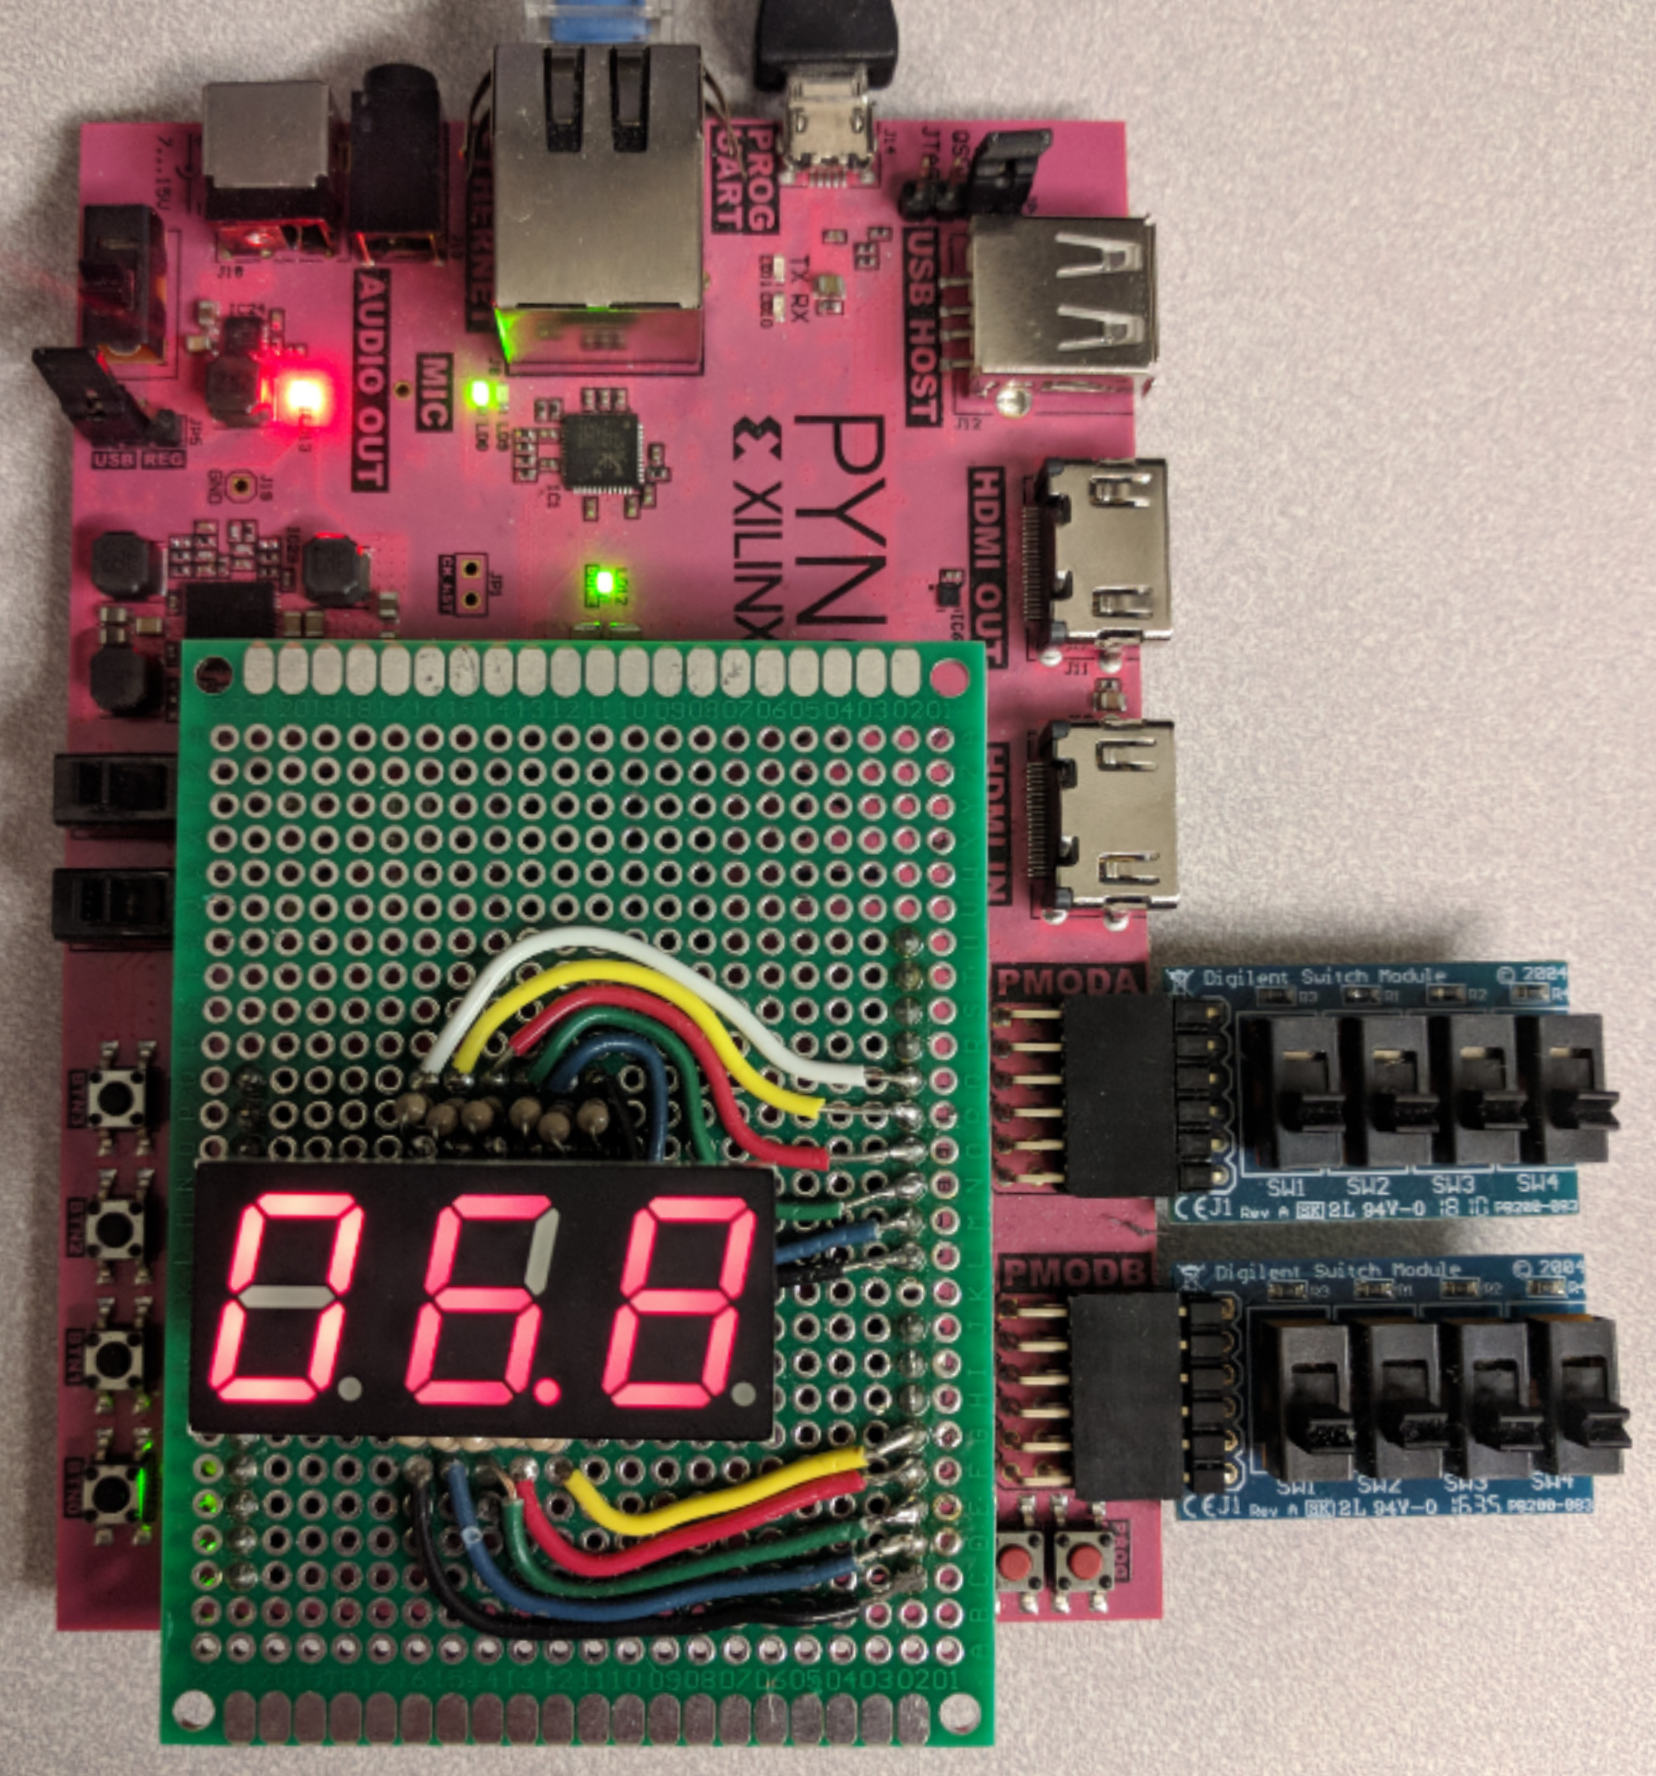
\includegraphics[width=.52\columnwidth,keepaspectratio]{figures/board}
	\caption{The PYNQ-Z1 Board Configured with a Stopwatch Partial Bitstream Generated by Maverick}
	\label{fig:board}
\end{figure}

We used the Maverick Jupyter notebook to run each of our benchmark designs through the full Maverick flow, all on the Zynq device's ARM CPU.
Following the bitstream generation of each design, an API added to the PYNQ system \cite{Goeders:2018} was used to partially reconfigure each design onto the Zynq's PL. 
Then, we functionally tested each design and verified their correct operation in hardware.
\figurename~\ref{fig:board} shows the PYNQ-Z1 board after it was partially reconfigured with a partial bitstream for the stopwatch design, which was generated by the Maverick flow. 

Additionally, we measured the run time for each benchmark design as it ran through each major step of the Maverick flow.
\figurename~\ref{fig:runtime} presents the run time results for each step running on the PYNQ-Z1's ARM CPU, which runs at 650 MHz. 
We also measured the run times for each step of the Maverick flow on a desktop computer with an Intel i7 860 CPU, which runs at 2.80 GHz.
For our benchmark designs, the Maverick flow executed from 6x to 11x slower on the PYNQ-Z1's ARM CPU.
Given the difference in CPU speeds and architectures, we found this to be unsurprising. 

\begin{figure}
	\centering
	\includegraphics[width=\columnwidth]{figures/runtime}
	\caption{Run Times on the PYNQ-Z1}
	\label{fig:runtime}
\end{figure}

Furthermore, we measured the peak memory usage for each major step of the Maverick flow as it executed on the PYNQ-Z1's ARM CPU. 
The iPython kernel and web server require roughly 120 MB of RAM, leaving 392 MB for the Maverick flow.
For the largest design we tested, Maverick required a maximum of 230 MB of RAM. 
Specifically, Yosys required 24 MB, the RapidSmith2-based programs 230 MB, and the Project X-Ray tools 14 MB of RAM.

To measure the resource utilization for the benchmarks compiled by the Maverick flow, we used the Vivado Design Interface (VDI) \cite{Townsend:2017b} (which was modified to support RM designs) to import each completed RM design into Vivado; we then measured the FPGA resource utilization for each.
Additionally, we compiled each RM design using only Vivado's PR flow and measured the resulting resource utilization for each design.
Table~\ref{tab:tab1} compares the resulting FPGA resource utilization from the Maverick flow and from Vivado's PR flow.
Note that the number of used LUTs in this table includes the LUTs in the netlist, LUTs used as route-throughs, and LUTs used as VCC or GND sources.

While Vivado was clearly able to produce better results, we still find these results to be promising and acceptable for use in a small embedded system.
The run times to fully compile the designs on the PYNQ-Z1's ARM processor were all on the order of a few minutes at most.
Additionally, the amount of RAM available for use by Maverick, roughly 392 MB, was almost double the RAM required for the designs we tested.
These results demonstrate the feasibility of running a stand-alone FPGA CAD tool flow on a resource-constrained platform such as the PYNQ-Z1, on which RMs can both be compiled and then programmed onto its own programmable fabric.

\begin{table}[t]
	\caption{Benchmark Design FPGA Resource Utilization}
	\label{tab:tab1}
	\begin{center}
		\begin{tabular}{|l|cc|cc|cc|}
			\toprule
			\multirow{2}{*}{}&\multicolumn{2}{c|}{Slices}&\multicolumn{2}{c|}{LUTs}&\multicolumn{2}{c|}{Flip-Flops}\\
			&Mav.&Viv.&Mav.&Viv.&Mav.&Viv.\\
			\midrule
			Register File & 28 & 21 &47 & 26 & 9 & 9\\
			RS232 Tx. & 53 & 42 & 174 & 114 & 55 & 48\\
			Stopwatch & 57 & 46 & 232 & 136 & 67 & 65\\
			Pattern Game & 79 & 58 & 319 & 187 & 117 & 109\\
			Timer Game & 105 & 73 & 589 & 233 & 128 & 127\\
			\midrule
			PR Region & \multicolumn{2}{c|}{400} & \multicolumn{2}{c|}{3200} & \multicolumn{2}{c|}{3200}\\
			xc7z020clg400-1 & \multicolumn{2}{c|}{13300} & \multicolumn{2}{c|}{106400} & \multicolumn{2}{c|}{106400}\\
			\bottomrule
		\end{tabular}
	\end{center}
\end{table}

\section{Conclusion and Future Work}
\label{sec:conclusion}

In this paper, we have presented the Maverick flow---a stand-alone CAD flow for RMs.
We demonstrated this by executing it on the PYNQ-Z1's ARM processor to compile a collection of Verilog designs to partial bitstreams.
These resulting bitstreams were all configured and verified in hardware on the PYNQ-Z1's FPGA fabric, demonstrating the feasibility of a single-chip system that can both compile HDL designs to bitstreams and then configure them onto its own programmable fabric.

Maverick uses a number of existing open source tools including Yosys, RapidSmith2, and Project X-Ray.  
We significantly modified some of these tools.
In particular, the existing RapidSmith2 import, packer, placer, and device model generation tools were all heavily modified to support PR, as was VDI.
Additionally, the Project X-Ray xc7Patch program was modified to create xc7PartialPatch, which functions with partial bitstreams.
New tools were also created as a part of this work, including a RapidSmith2-based router and a RapidSmith2 FASM file generator.
Other software was also created to interface the various pieces of Maverick to one another, creating a turnkey system.

We see several potential future opportunities for Maverick.
Firstly, we are preparing it for open source distribution so it can be used and extended by others in the community.
Maverick could also be enhanced to work with other Xilinx architectures beyond 7-Series, such as the Zynq UltraScale+.
There is nothing in the tools comprising Maverick which would prevent them from doing so.
In fact, several of these already have support for devices beyond 7-Series.
Another extension to Maverick would be to support multiple PR regions within the same device, a modest change to the existing system.
Maverick could also be updated to support additional primitives in 7-Series devices as Yosys and Project X-Ray expand their supported set.
Furthermore, we plan on exploring the use of Maverick in an educational setting to teach digital design, providing instructional materials, CAD tools, analysis and visualization tools, and a hardware platform in one PYNQ system.


% references section
\bibliographystyle{IEEEtran}
\bibliography{IEEEabrv,references}

\end{document}
